\section{Results}
\label{sec:results}

\subsection{Main comparison (RQ2)}
Table~\ref{tab:main} reports the primary set (861 HotpotQA bridge questions) with gpt-4o-mini as generator. Among the methods that make no LLM call, SES-RAG attains the highest gold-complete rate (63.1\%) and F1 (54.8\%). Table~\ref{tab:tests} gives the paired comparisons. SES-RAG is significantly better than Naive and Hybrid RAG on both metrics (about +10 points gold-complete and +5.7 points F1, Holm $p<0.001$), and better than the $\mu{=}0$ control and G-Retriever-lite on gold-complete retrieval (+4.4 and +4.2 points, Holm $p\le 0.004$). Its leads over GraphRAG-lite and SpectRAG-lite (+2.9 and +2.4 points gold-complete, +2.7 and +1.5 points F1) and its F1 leads over the control and G-Retriever-lite are not significant after correction. The LLM-driven IRCoT-lite is clearly ahead of SES-RAG ($-11.3$ points gold-complete, $-7.1$ points F1). The pre-declared criterion, that SES-RAG beats every baseline on both metrics, is therefore \emph{not} met. All of these systems remain far from the gold-first oracle (71.0\% F1).

\begin{table*}[t]
\centering
\caption{HotpotQA bridge questions ($n=861$), generator gpt-4o-mini, 600-token budget. Mean with 95\% bootstrap CI. LLM calls = query-time LLM calls before answering.}
\label{tab:main}
\small
\resizebox{\textwidth}{!}{%
\begin{tabular}{lccccc}
\toprule
System & Gold-complete (\%) & F1 (\%) & Judged acc. (\%) & Abstain (\%) & LLM calls \\
\midrule
Naive RAG & 52.4\,{\scriptsize[49.1,55.9]} & 49.1\,{\scriptsize[45.9,52.2]} & 53.2\,{\scriptsize[49.8,56.6]} & 30.5\,{\scriptsize[27.5,33.7]} & 0 \\
Hybrid RAG & 53.2\,{\scriptsize[49.9,56.6]} & 49.1\,{\scriptsize[45.9,52.1]} & 53.2\,{\scriptsize[49.7,56.6]} & 31.7\,{\scriptsize[28.7,34.8]} & 0 \\
Hybrid+Expand ($\mu{=}0$) & 58.7\,{\scriptsize[55.4,62.0]} & 53.0\,{\scriptsize[49.9,56.0]} & 57.4\,{\scriptsize[53.9,60.6]} & 28.6\,{\scriptsize[25.6,31.6]} & 0 \\
GraphRAG-lite & 60.2\,{\scriptsize[56.8,63.4]} & 52.1\,{\scriptsize[49.0,55.1]} & 56.2\,{\scriptsize[52.7,59.5]} & 28.3\,{\scriptsize[25.4,31.4]} & 0 \\
SpectRAG-lite & 60.6\,{\scriptsize[57.4,64.0]} & 53.3\,{\scriptsize[50.1,56.4]} & 57.0\,{\scriptsize[53.7,60.4]} & 27.4\,{\scriptsize[24.4,30.4]} & 0 \\
G-Retriever-lite & 58.9\,{\scriptsize[55.6,62.3]} & 53.0\,{\scriptsize[49.7,56.0]} & 57.1\,{\scriptsize[53.8,60.4]} & 28.6\,{\scriptsize[25.4,31.5]} & 0 \\
IRCoT-lite & 74.3\,{\scriptsize[71.4,77.4]} & 61.9\,{\scriptsize[58.9,64.8]} & 66.9\,{\scriptsize[63.6,70.0]} & 19.5\,{\scriptsize[17.0,22.1]} & 3 \\
\textbf{SES-RAG} & 63.1\,{\scriptsize[59.9,66.3]} & 54.8\,{\scriptsize[51.4,57.7]} & 59.7\,{\scriptsize[56.2,63.0]} & 25.1\,{\scriptsize[22.3,28.1]} & 0 \\
IRCoT+SES & 75.0\,{\scriptsize[72.2,77.8]} & 61.6\,{\scriptsize[58.4,64.5]} & 66.2\,{\scriptsize[63.0,69.3]} & 18.5\,{\scriptsize[16.0,21.1]} & 3 \\
\midrule
Gold-first oracle & 100.0\,{\scriptsize[100.0,100.0]} & 71.0\,{\scriptsize[68.2,73.6]} & 75.7\,{\scriptsize[72.7,78.5]} & 9.6\,{\scriptsize[7.8,11.6]} & -- \\
\bottomrule
\end{tabular}}
\end{table*}
\begin{table}[t]
\centering
\caption{SES-RAG minus each baseline, primary set, gpt-4o-mini (paired one-sided bootstrap, Holm-corrected over the 14 comparisons).}
\label{tab:tests}
\small
\resizebox{\columnwidth}{!}{%
\begin{tabular}{llccc}
\toprule
Baseline & Metric & $\Delta$ (pts) & 95\% CI & Holm $p$ \\
\midrule
Naive RAG & Gold-complete & +10.7 & [+7.5, +13.8] & $<$0.001 \\
Naive RAG & F1 & +5.7 & [+3.2, +8.2] & $<$0.001 \\
Hybrid RAG & Gold-complete & +9.9 & [+6.8, +12.9] & $<$0.001 \\
Hybrid RAG & F1 & +5.7 & [+3.3, +8.3] & $<$0.001 \\
Hybrid+Expand ($\mu{=}0$) & Gold-complete & +4.4 & [+1.9, +7.1] & 0.004 \\
Hybrid+Expand ($\mu{=}0$) & F1 & +1.8 & [-0.4, +4.1] & 0.278 \\
GraphRAG-lite & Gold-complete & +2.9 & [+0.2, +5.6] & 0.136 \\
GraphRAG-lite & F1 & +2.7 & [+0.5, +4.9] & 0.062 \\
SpectRAG-lite & Gold-complete & +2.4 & [-0.1, +5.0] & 0.209 \\
SpectRAG-lite & F1 & +1.5 & [-0.7, +3.8] & 0.278 \\
G-Retriever-lite & Gold-complete & +4.2 & [+1.6, +6.9] & 0.002 \\
G-Retriever-lite & F1 & +1.9 & [-0.4, +4.1] & 0.278 \\
IRCoT-lite & Gold-complete & -11.3 & [-14.8, -7.9] & 1.000 \\
IRCoT-lite & F1 & -7.1 & [-9.9, -4.3] & 1.000 \\
\bottomrule
\end{tabular}}
\end{table}

\subsection{Generator robustness}
Table~\ref{tab:gen} repeats the F1 comparison for all four generators on the identical contexts. The ordering of the point estimates of the systems shown is the same for every generator: Naive $\approx$ Hybrid $<$ Hybrid+Expand $\approx$ SpectRAG-lite $<$ SES-RAG $<$ IRCoT-lite $<$ oracle. SES-RAG improves on Hybrid RAG by 5.7, 6.5, 5.8 and 4.0 F1 points for gpt-4o-mini, gpt-4o, claude-sonnet-5-5 and claude-haiku-5-5 (all 95\% intervals exclude zero), and is below IRCoT-lite by 7.1 to 10.3 points. The gain therefore does not depend on a particular generator.

\begin{table*}[t]
\centering
\caption{Answer F1 (\%) by generator on the primary set (same contexts, different generators).}
\label{tab:gen}
\small
\resizebox{\textwidth}{!}{%
\begin{tabular}{lccccccc}
\toprule
Generator & Naive RAG & Hybrid RAG & Hybrid+Expand ($\mu{=}0$) & SpectRAG-lite & IRCoT-lite & SES-RAG & Gold-first oracle \\
\midrule
gpt-4o-mini & 49.1 & 49.1 & 53.0 & 53.3 & 61.9 & 54.8 & 71.0 \\
gpt-4o & 49.5 & 50.0 & 53.5 & 54.0 & 64.1 & 56.5 & 74.8 \\
claude-sonnet-5-5 & 53.1 & 53.3 & 56.0 & 56.6 & 68.4 & 59.1 & 78.5 \\
claude-haiku-5-5 & 48.6 & 49.8 & 52.4 & 52.6 & 64.1 & 53.8 & 74.5 \\
\bottomrule
\end{tabular}}
\end{table*}

\subsection{Bridge failure and answer quality (RQ1)}
Table~\ref{tab:link} splits all contexts by whether they contain all gold paragraphs. With a complete context the generators answer correctly 77.8--87.5\% of the time (judged) and reach 72.6--79.9\% F1 while abstaining on 2.4--8.2\% of questions. With a bridge-failed context judged accuracy falls to 22.3--27.0\%, F1 to 19.2--24.1\%, and the generators abstain on 53.4--63.4\% of questions. Improving retrieval completeness is thus the primary lever for answer quality on bridge questions, whichever generator is used (Fig.~\ref{fig:link}). This comparison is observational and the contexts are pooled over eight systems, so it should be read as an association. It is not an artefact of question difficulty: comparing systems on the \emph{same} question (question fixed effects), a complete context raises F1 by 0.48, 0.54, 0.56 and 0.57 for the four generators, nearly identical to the raw gaps of 0.49, 0.54, 0.56 and 0.57. The gold-first oracle provides a more interventional reference: giving every system the gold paragraphs raises F1 from 54.8\% (SES-RAG) to 71.0\% with gpt-4o-mini.

\begin{table}[t]
\centering
\caption{Outcome by whether the context contains all gold paragraphs (pooled over the eight non-oracle systems on the primary set).}
\label{tab:link}
\small
\resizebox{\columnwidth}{!}{%
\begin{tabular}{llrccc}
\toprule
Generator & Context & $n$ & Judged acc. (\%) & F1 (\%) & Abstain (\%) \\
\midrule
gpt-4o-mini & bridge-failed & 2744 & 27.0 & 24.1 & 56.5 \\
gpt-4o-mini & complete & 4144 & 77.8 & 72.6 & 8.2 \\
gpt-4o & bridge-failed & 2744 & 24.9 & 21.8 & 63.4 \\
gpt-4o & complete & 4144 & 81.9 & 75.7 & 7.5 \\
claude-sonnet-5-5 & bridge-failed & 2744 & 26.4 & 23.4 & 53.4 \\
claude-sonnet-5-5 & complete & 4144 & 87.5 & 79.9 & 2.4 \\
claude-haiku-5-5 & bridge-failed & 2744 & 22.3 & 19.2 & 56.3 \\
claude-haiku-5-5 & complete & 4144 & 82.3 & 75.7 & 5.5 \\
\bottomrule
\end{tabular}}
\end{table}

\begin{figure}[t]
\centering
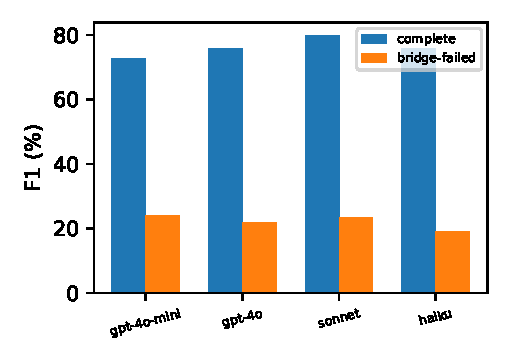
\includegraphics[width=\columnwidth]{figs/fig_link}
\caption{F1 by generator when the context is complete or bridge-failed (primary set, eight systems pooled).}
\label{fig:link}
\end{figure}

\subsection{Is spectral connectivity the active ingredient? (RQ3)}
Table~\ref{tab:abl} replaces the $\lambda_2$ term by alternatives, keeping the weight $\mu$ tuned for the normalised $\lambda_2$. The unnormalised $\lambda_2$ has a different scale, so its best $\mu$ differs; we treat the comparison as indicative. Removing the term altogether ($\mu{=}0$) costs 4.4 gold-complete points, confirming that rewarding connectivity helps. But the \emph{number of connected components} (a count, no eigenvalues) and the \emph{unnormalised} $\lambda_2$ score 2.2 and 2.8 points higher gold-complete (uncorrected intervals above zero; Holm-corrected over the eight ablation comparisons $p=0.11$, so not significant), with F1 differences within noise, and a plain density term is equivalent. Only the removal of the term ($\mu{=}0$) is significantly worse (Holm $p=0.002$ for gold-complete). The comparison is indicative: the component-count objective is integer-valued, so a common $\mu$ is not on a common scale. Sensitivity to $\mu$ (Fig.~\ref{fig:mu}) shows the same picture: the unnormalised variant peaks at 68.6\% at $\mu{=}1$, whereas the normalised variant peaks at 63.1\% at $\mu{=}0.25$. This sweep was run on the primary set after the protocol was fixed; its maximum over seven values of $\mu$ is optimistic, and it is exploratory. We conclude that the benefit comes from a connectivity reward in general, and that spectral quantities offer no demonstrated advantage over simpler ones here.

\begin{table}[t]
\centering
\caption{Ablations of the selection objective (primary set, gpt-4o-mini). $\Delta$ = variant minus SES-RAG, 95\% CI.}
\label{tab:abl}
\small
\resizebox{\columnwidth}{!}{%
\begin{tabular}{lcccc}
\toprule
Variant & Gold-complete & $\Delta$ & F1 & $\Delta$ \\
\midrule
SES-RAG (norm.\ $\lambda_2$) & 63.1 & -- & 54.8 & -- \\
Hybrid+Expand ($\mu{=}0$) & 58.7 & -4.4 [-7.1,-1.9] & 53.0 & -1.8 [-4.1,+0.4] \\
SES, component count & 65.3 & +2.2 [+0.5,+3.9] & 55.8 & +1.0 [-0.6,+2.7] \\
SES, density term & 62.5 & -0.6 [-3.1,+1.9] & 53.9 & -0.9 [-3.1,+1.2] \\
SES, raw $\lambda_2$ & 65.9 & +2.8 [+0.7,+5.0] & 55.4 & +0.6 [-1.3,+2.4] \\
\bottomrule
\end{tabular}}
\end{table}

\begin{figure}[t]
\centering
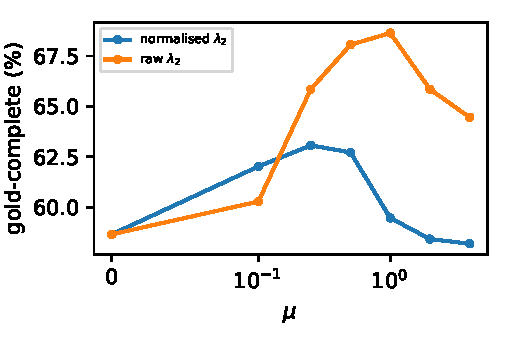
\includegraphics[width=\columnwidth]{figs/fig_mu}
\caption{Gold-complete rate of SES-RAG versus $\mu$ for the normalised and unnormalised $\lambda_2$ (primary set, exploratory sensitivity analysis).}
\label{fig:mu}
\end{figure}

\subsection{Token budget}
Figure~\ref{fig:budget} shows gold-complete retrieval for budgets from 300 to 1{,}500 tokens. SES-RAG has the highest point estimate among LLM-free methods at every budget (no intervals were computed for this sweep, and $\mu$ was not re-tuned per budget), with the largest margins at tight budgets (47.3\% at 300 tokens versus 41.0\% for the next best, GraphRAG-lite), and the curves converge as the budget grows (80.7\% vs.\ 79.9\% for SpectRAG-lite at 1{,}500, where the iterative baseline's context uses only about 1{,}000 of the 1{,}500 tokens). Connectivity-aware packing matters most when the budget forces a choice among candidates.

\begin{figure}[t]
\centering
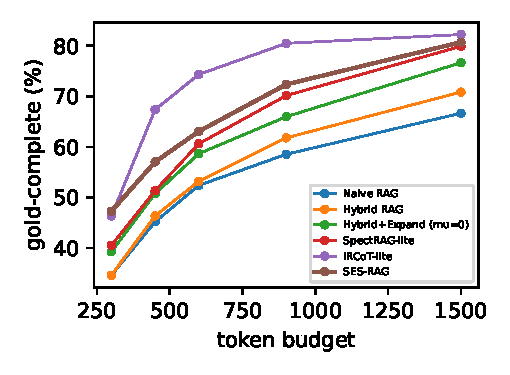
\includegraphics[width=\columnwidth]{figs/fig_budget}
\caption{Gold-complete rate versus token budget (primary set).}
\label{fig:budget}
\end{figure}

\subsection{Extension: iterative retrieval with connectivity-aware packing}
IRCoT+SES adds the iterative-retrieval candidates to the SES pool and packs the budget with the same rule (Section~\ref{sec:method}). On the development and exploration questions it improved gold-complete retrieval from 74.0\% to 77.0\%, but on the primary set it did not: 75.0\% vs.\ 74.3\% gold-complete (+0.7 points, 95\% CI $-2.0$ to $+3.4$) and 61.6\% vs.\ 61.9\% F1 ($-0.3$, CI $-2.6$ to $+2.0$). It is better than SES-RAG alone (+12.0 gold-complete, +6.8 F1 points), so the retrieval of the bridge, not the packing, accounts for IRCoT's advantage. On MuSiQue IRCoT+SES is \emph{worse} than IRCoT-lite in gold-complete rate ($-4.4$ points, 95\% CI $-7.2$ to $-1.6$) and not better on 2WikiMultiHopQA ($-0.4$, CI $-4.0$ to $+3.4$).

\subsection{Where SES-RAG loses}
The candidate pool contains every gold paragraph for 90.8\% of the primary questions, and at least one gold paragraph is a retrieval seed for 99.1\%. SES-RAG's context is complete for 63.1\%: about 28 points are lost at selection (the gold paragraphs were in the pool but not chosen) and about 9 points because the pool lacked one. Since the pool has 100 candidates for about five context slots, pool recall is a loose ceiling. In 73.3\% of questions the two gold paragraphs are directly linked in the graph.

\subsection{Dependence on the graph and transfer (RQ4)}
\paragraph{Without title-mention edges.}
We rebuilt the graph with the mention signal removed and re-tuned the parametrised systems on the development and exploration questions. Table~\ref{tab:nomention} gives gold-complete rates on the primary set. SES-RAG falls from 63.1\% to 57.5\%, no better than the $\mu{=}0$ control (58.3\%; difference $-0.8$ points, 95\% CI $-3.4$ to $+1.7$) or G-Retriever-lite (58.4\%). On this graph the re-tuned mixing weight of SpectRAG-lite is zero, which makes its selections identical to the control's, so it is not an independent comparison. GraphRAG-lite and IRCoT-lite do not read the graph and are unchanged. SES-RAG still exceeds Hybrid and Naive RAG by 4.3 and 5.1 points because the pool is expanded through the remaining entity and similarity edges; it is the connectivity reward on top of the expanded pool that no longer helps. We did not test an interaction between the graph and the reward statistically, and the spectral coordinates of SpectRAG-lite in this run use the largest connected component only. With gpt-4o-mini, SES-RAG reaches 51.5\% F1 against 52.6\% for the control and SpectRAG-lite on the same questions. The connectivity reward needs a graph that actually links bridge passages.

\begin{table}[t]
\centering
\caption{Primary set with and without title-mention edges in the graph: gold-complete rate (\%) and, where answered with gpt-4o-mini, F1 (\%).}
\label{tab:nomention}
\small
\resizebox{\columnwidth}{!}{%
\begin{tabular}{lccc}
\toprule
System & Gold-complete, with & Gold-complete, without & F1, without \\
\midrule
Naive RAG & 52.4 & 52.4 & -- \\
Hybrid RAG & 53.2 & 53.2 & -- \\
Hybrid+Expand ($\mu{=}0$) & 58.7 & 58.3 & 52.6 \\
GraphRAG-lite & 60.2 & 60.2 & -- \\
SpectRAG-lite & 60.6 & 58.3 & 52.6 \\
G-Retriever-lite & 58.9 & 58.4 & -- \\
IRCoT-lite & 74.3 & 74.3 & -- \\
SES-RAG & 63.1 & 57.5 & 51.5 \\
\bottomrule
\end{tabular}}
\end{table}

\paragraph{2WikiMultiHopQA.}
On 500 compositional and inference questions, with every setting frozen on HotpotQA and no re-tuning, SES-RAG's gold-complete rate is 43.2\%, against 23.8\% for Hybrid RAG and 33.8--34.8\% for SpectRAG-lite and GraphRAG-lite (Table~\ref{tab:2wiki}). The gold-complete gains over every LLM-free baseline (+8.4 to +19.4 points) are significant after Holm correction. F1 improves by 1.8 to 5.8 points, significantly for all but GraphRAG-lite. IRCoT-lite reaches 65.6\% gold-complete and 27.2\% F1 (SES-RAG: 21.0\%), against a ceiling of 32.6\% F1 for the gold-first oracle. The corpus here is small (5{,}173 paragraphs, many shared across questions), so absolute completeness is not comparable with HotpotQA's. At 600 tokens even the oracle fits all gold paragraphs for only 84.4\% of these questions.

\begin{table}[t]
\centering
\caption{2WikiMultiHopQA ($n=500$ questions, settings frozen on HotpotQA), gpt-4o-mini.}
\label{tab:2wiki}
\small
\resizebox{\columnwidth}{!}{%
\begin{tabular}{lcccc}
\toprule
System & Gold-complete (\%) & F1 (\%) & Judged acc. (\%) & LLM calls \\
\midrule
Naive RAG & 26.8\,{\scriptsize[22.8,30.8]} & 16.0\,{\scriptsize[13.1,18.9]} & 15.4\,{\scriptsize[12.2,18.6]} & 0 \\
Hybrid RAG & 23.8\,{\scriptsize[20.2,27.4]} & 15.1\,{\scriptsize[12.4,18.0]} & 14.2\,{\scriptsize[11.2,17.2]} & 0 \\
Hybrid+Expand ($\mu{=}0$) & 29.2\,{\scriptsize[25.2,33.2]} & 16.8\,{\scriptsize[14.0,19.7]} & 16.8\,{\scriptsize[13.6,20.2]} & 0 \\
GraphRAG-lite & 34.8\,{\scriptsize[30.6,39.2]} & 19.1\,{\scriptsize[16.0,22.4]} & 20.0\,{\scriptsize[16.6,23.6]} & 0 \\
SpectRAG-lite & 33.8\,{\scriptsize[29.6,38.0]} & 18.4\,{\scriptsize[15.4,21.6]} & 18.2\,{\scriptsize[15.0,21.6]} & 0 \\
G-Retriever-lite & 30.4\,{\scriptsize[26.4,34.6]} & 17.0\,{\scriptsize[14.0,20.0]} & 16.8\,{\scriptsize[13.6,20.2]} & 0 \\
IRCoT-lite & 65.6\,{\scriptsize[61.6,69.8]} & 27.2\,{\scriptsize[23.6,30.6]} & 28.4\,{\scriptsize[24.4,32.2]} & 3 \\
\textbf{SES-RAG} & 43.2\,{\scriptsize[38.8,47.6]} & 21.0\,{\scriptsize[17.8,24.1]} & 21.2\,{\scriptsize[17.6,24.8]} & 0 \\
IRCoT+SES & 65.2\,{\scriptsize[61.0,69.4]} & 27.2\,{\scriptsize[23.5,30.7]} & 28.6\,{\scriptsize[24.6,32.4]} & 3 \\
\midrule
Gold-first oracle & 84.4\,{\scriptsize[81.2,87.6]} & 32.6\,{\scriptsize[28.9,36.2]} & 34.2\,{\scriptsize[30.0,38.0]} & -- \\
\bottomrule
\end{tabular}}
\end{table}

Table~\ref{tab:transfer_tests} lists the paired comparisons for both external datasets.

\paragraph{MuSiQue.}
MuSiQue questions need two to four hops and every method struggles (Table~\ref{tab:musique}): gold-complete rates are 16--22\% for all LLM-free systems and SES-RAG (21.4\%) is indistinguishable from the control, Naive RAG, GraphRAG-lite, SpectRAG-lite and G-Retriever-lite; it improves only on Hybrid RAG (+5.0 points, Holm $p=0.003$). IRCoT-lite is 10 points ahead (31.8\%). The connectivity reward therefore does not transfer to these deeper chains at this budget.

\begin{table}[t]
\centering
\caption{MuSiQue ($n=500$ questions, settings frozen on HotpotQA), gpt-4o-mini.}
\label{tab:musique}
\small
\resizebox{\columnwidth}{!}{%
\begin{tabular}{lcccc}
\toprule
System & Gold-complete (\%) & F1 (\%) & Judged acc. (\%) & LLM calls \\
\midrule
Naive RAG & 21.2\,{\scriptsize[17.6,24.8]} & 16.3\,{\scriptsize[13.3,19.5]} & 18.2\,{\scriptsize[14.8,21.6]} & 0 \\
Hybrid RAG & 16.4\,{\scriptsize[13.2,19.8]} & 13.3\,{\scriptsize[10.7,16.1]} & 14.4\,{\scriptsize[11.4,17.6]} & 0 \\
Hybrid+Expand ($\mu{=}0$) & 21.4\,{\scriptsize[18.0,25.0]} & 16.9\,{\scriptsize[14.0,20.1]} & 18.4\,{\scriptsize[15.0,22.0]} & 0 \\
GraphRAG-lite & 20.8\,{\scriptsize[17.4,24.4]} & 16.8\,{\scriptsize[13.9,20.1]} & 17.8\,{\scriptsize[14.6,21.2]} & 0 \\
SpectRAG-lite & 21.0\,{\scriptsize[17.4,24.6]} & 15.8\,{\scriptsize[13.0,18.8]} & 17.4\,{\scriptsize[14.2,20.8]} & 0 \\
G-Retriever-lite & 21.8\,{\scriptsize[18.2,25.4]} & 15.9\,{\scriptsize[13.1,19.0]} & 17.6\,{\scriptsize[14.4,20.8]} & 0 \\
IRCoT-lite & 31.8\,{\scriptsize[27.6,35.8]} & 24.2\,{\scriptsize[20.8,27.8]} & 25.6\,{\scriptsize[22.0,29.6]} & 3 \\
\textbf{SES-RAG} & 21.4\,{\scriptsize[17.8,25.0]} & 16.6\,{\scriptsize[13.6,19.6]} & 18.0\,{\scriptsize[14.6,21.4]} & 0 \\
IRCoT+SES & 27.4\,{\scriptsize[23.4,31.2]} & 22.2\,{\scriptsize[18.9,25.7]} & 24.2\,{\scriptsize[20.4,28.2]} & 3 \\
\midrule
Gold-first oracle & 92.4\,{\scriptsize[90.2,94.8]} & 32.8\,{\scriptsize[29.2,36.7]} & 34.6\,{\scriptsize[30.6,38.6]} & -- \\
\bottomrule
\end{tabular}}
\end{table}
\begin{table}[t]
\centering
\caption{SES-RAG minus each baseline on the external datasets (gpt-4o-mini; $\Delta$ in points, 95\% CI, Holm $p$ over the 14 comparisons per dataset).}
\label{tab:transfer_tests}
\small
\resizebox{\columnwidth}{!}{%
\begin{tabular}{llllcc}
\toprule
Dataset & Baseline & Metric & $\Delta$ & 95\% CI & Holm $p$ \\
\midrule
MuSiQue & Naive RAG & Gold-complete & +0.2 & [-2.8, +3.0] & 1.000 \\
MuSiQue & Naive RAG & F1 & +0.2 & [-2.2, +2.6] & 1.000 \\
MuSiQue & Hybrid RAG & Gold-complete & +5.0 & [+2.4, +7.8] & 0.003 \\
MuSiQue & Hybrid RAG & F1 & +3.2 & [+0.6, +5.8] & 0.094 \\
MuSiQue & Hybrid+Expand ($\mu{=}0$) & Gold-complete & +0.0 & [-2.2, +2.2] & 1.000 \\
MuSiQue & Hybrid+Expand ($\mu{=}0$) & F1 & -0.4 & [-2.5, +1.7] & 1.000 \\
MuSiQue & GraphRAG-lite & Gold-complete & +0.6 & [-2.0, +3.2] & 1.000 \\
MuSiQue & GraphRAG-lite & F1 & -0.3 & [-2.6, +2.0] & 1.000 \\
MuSiQue & SpectRAG-lite & Gold-complete & +0.4 & [-2.0, +2.8] & 1.000 \\
MuSiQue & SpectRAG-lite & F1 & +0.7 & [-1.7, +3.1] & 1.000 \\
MuSiQue & G-Retriever-lite & Gold-complete & -0.4 & [-2.8, +2.0] & 1.000 \\
MuSiQue & G-Retriever-lite & F1 & +0.6 & [-1.4, +2.7] & 1.000 \\
MuSiQue & IRCoT-lite & Gold-complete & -10.4 & [-14.2, -6.8] & 1.000 \\
MuSiQue & IRCoT-lite & F1 & -7.7 & [-10.9, -4.5] & 1.000 \\
2Wiki & Naive RAG & Gold-complete & +16.4 & [+12.8, +20.0] & $<$0.001 \\
2Wiki & Naive RAG & F1 & +5.0 & [+2.8, +7.4] & $<$0.001 \\
2Wiki & Hybrid RAG & Gold-complete & +19.4 & [+15.8, +23.2] & $<$0.001 \\
2Wiki & Hybrid RAG & F1 & +5.8 & [+3.4, +8.4] & $<$0.001 \\
2Wiki & Hybrid+Expand ($\mu{=}0$) & Gold-complete & +14.0 & [+10.8, +17.2] & $<$0.001 \\
2Wiki & Hybrid+Expand ($\mu{=}0$) & F1 & +4.1 & [+2.1, +6.3] & 0.001 \\
2Wiki & GraphRAG-lite & Gold-complete & +8.4 & [+5.0, +12.0] & $<$0.001 \\
2Wiki & GraphRAG-lite & F1 & +1.8 & [-0.7, +4.3] & 0.201 \\
2Wiki & SpectRAG-lite & Gold-complete & +9.4 & [+6.2, +12.8] & $<$0.001 \\
2Wiki & SpectRAG-lite & F1 & +2.5 & [+0.3, +4.8] & 0.043 \\
2Wiki & G-Retriever-lite & Gold-complete & +12.8 & [+9.6, +16.2] & $<$0.001 \\
2Wiki & G-Retriever-lite & F1 & +4.0 & [+1.7, +6.2] & 0.001 \\
2Wiki & IRCoT-lite & Gold-complete & -22.4 & [-27.2, -17.4] & 1.000 \\
2Wiki & IRCoT-lite & F1 & -6.2 & [-9.6, -2.9] & 1.000 \\
\bottomrule
\end{tabular}}
\end{table}
\begin{table}[t]
\centering
\caption{External datasets by generator: gold-complete (\%) is generator-independent; F1 (\%) differs by generator.}
\label{tab:extgen}
\small
\resizebox{\columnwidth}{!}{%
\resizebox{\columnwidth}{!}{%
\begin{tabular}{llccccc}
\toprule
Dataset & Generator & Naive & SpectRAG-lite & IRCoT-lite & SES-RAG & Oracle \\
\midrule
MuSiQue & gpt-4o-mini & 21.2 / 16.3 & 21.0 / 15.8 & 31.8 / 24.2 & 21.4 / 16.6 & 92.4 / 32.8 \\
MuSiQue & claude-sonnet-5-5 & 21.2 / 20.4 & 21.0 / 20.2 & 31.8 / 30.1 & 21.4 / 19.8 & 92.4 / 47.6 \\
2Wiki & gpt-4o-mini & 26.8 / 16.0 & 33.8 / 18.4 & 65.6 / 27.2 & 43.2 / 21.0 & 84.4 / 32.6 \\
2Wiki & claude-sonnet-5-5 & 26.8 / 20.4 & 33.8 / 23.1 & 65.6 / 40.2 & 43.2 / 29.3 & 84.4 / 50.4 \\
\bottomrule
\end{tabular}}}
\end{table}

Table~\ref{tab:extgen} repeats the comparison with claude-sonnet-5-5 as generator. The ordering of SES-RAG, SpectRAG-lite and IRCoT-lite is unchanged, and on 2WikiMultiHopQA absolute F1 is higher for Claude (IRCoT-lite 40.2\%, oracle 50.4\%) than for gpt-4o-mini (27.2\%, 32.6\%), so the oracle abstention ceiling noted below is generator-specific.

\paragraph{A caveat on answer metrics for the external datasets.} Even when the gold paragraphs are the whole context, gpt-4o-mini abstains on 48\% of 2WikiMultiHopQA and 48\% of MuSiQue questions (9.6\% on HotpotQA), so the labelled supporting paragraphs are often not enough for the model to commit to an answer. F1 on these datasets is therefore capped well below HotpotQA's (oracle F1: 32.6\% and 32.8\%), and we regard the gold-complete rate as the more reliable metric there. Hybrid RAG is also below Naive RAG on both external datasets, so fusion with BM25 is not uniformly helpful in this setting.


\subsection{Cost}
Selecting the context with SES-RAG takes 3.7\,ms per question on a CPU, given the shared candidate pool, and requires no LLM call; the corresponding selection step takes 0.03\,ms for Hybrid RAG and 0.2\,ms for SpectRAG-lite. The timings exclude pool construction, BM25 scoring and graph building, which all graph-based systems share. IRCoT-lite needs three sequential LLM calls (plus three embedding calls) per question before the answer is generated.
